\section{Пример добавления в документ рисунка из файла, созданного сторонней программой}
\sectionmark{Пример добавления в документ рисунка из файла}

\subsection{Один рисунок}

На рисунке~\ref{p:func_in2_1} приведена функциональная 
схема измерителя напряжения ИН2. В книге \cite{gussens} можно найти дополнительные сведения по включению рисунков в документ.


\begin{figure}[H]
  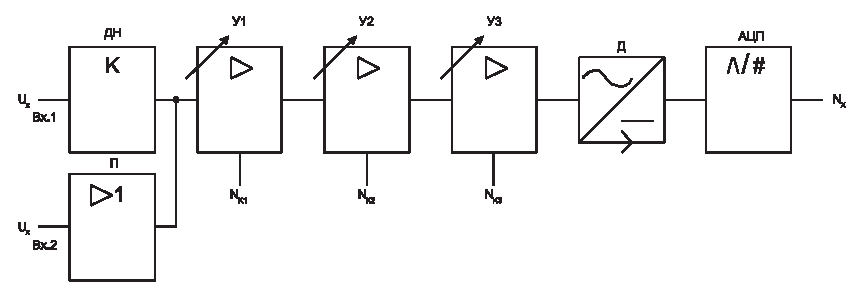
\includegraphics[width=1\textwidth]{./about/func_in}
  \caption{Функциональная схема измерителя напряжения ИН2, необходимая для демонстрации возможностей включения рисунков и корректного переноса подрисуночной подписи} \label{p:func_in2_1}
\end{figure}


\begin{figure}[H]
  \centering
  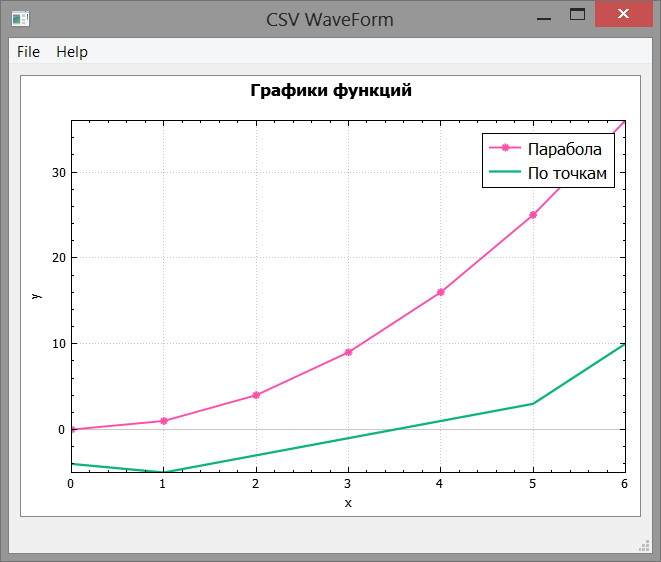
\includegraphics[width=0.7\textwidth]{./about/scv_waveform/csv_waveform.jpg}
  \caption{Графики каких-то функций, открытые бесплатной программой с открытым исходным кодом 'CSV WaveForm' и доступной по адресу https://github.com/yrasik/csv\_waveform} \label{pic:scv_waveform}
\end{figure}



\subsection{Два рисунка в ряд }

\begin{figure}[H]
\begin{minipage}[h]{0.49\linewidth}
\center{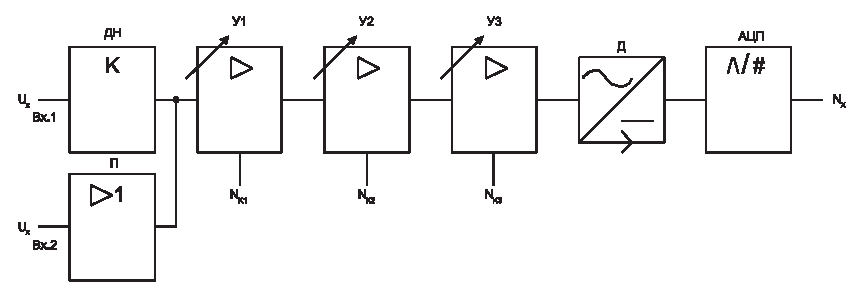
\includegraphics[width=0.7\linewidth]{./about/func_in} \\ а)}
\end{minipage}
\hfill
\begin{minipage}[h]{0.49\linewidth}
\center{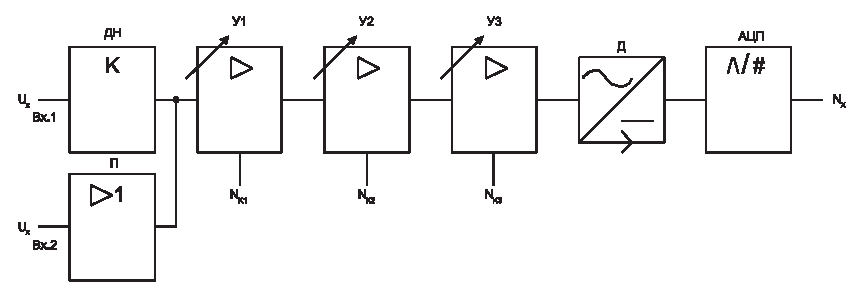
\includegraphics[width=0.7\linewidth]{./about/func_in} \\ б)}
\end{minipage}
\caption{Зависимость сигнала от шума для данных.}
\label{ris:image1}
\end{figure}



\newpage
\subsection{Два рисунка в ряд с разными подписями}


\begin{figure}[H]
\begin{center}
  \captionsetup{width=60mm}%
\begin{minipage}[h]{0.4\linewidth}
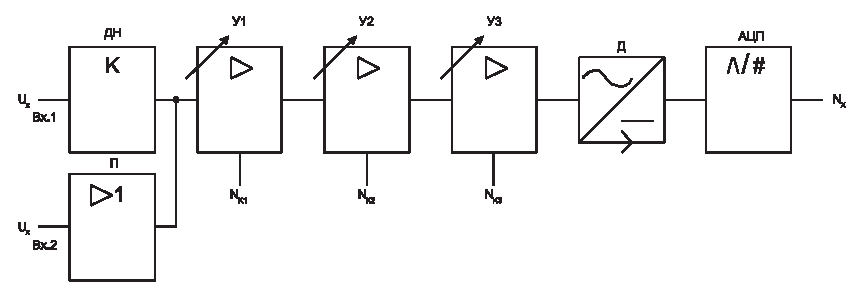
\includegraphics[width=1\linewidth]{./about/func_in}
\caption{Исходное изображение.} %% подпись к рисунку
\label{ris:experimoriginal} %% метка рисунка для ссылки на него
\end{minipage}
\hfill
\begin{minipage}[h]{0.4\linewidth}
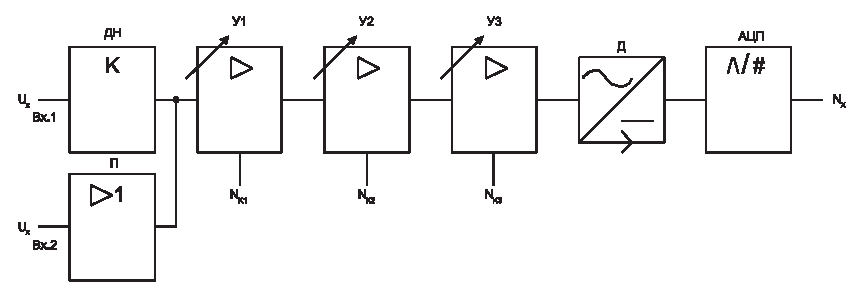
\includegraphics[width=1\linewidth]{./about/func_in}
\caption{Закодированное изображение.}
\label{ris:experimcoded}
\end{minipage}
\end{center}
\end{figure}



\begin{figure}[H]
\begin{center}
  \captionsetup{width=50mm,
      %margin={250mm,-250mm}
      }%
\begin{minipage}[h]{0.3\linewidth}
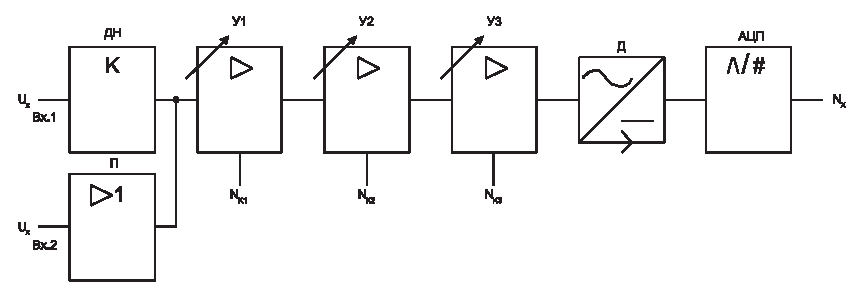
\includegraphics[width=1\linewidth]{./about/func_in}
\caption{} %% подпись к рисунку
\label{ris:expe1} %% метка рисунка для ссылки на него
\end{minipage}
\hfill
\begin{minipage}[h]{0.3\linewidth}
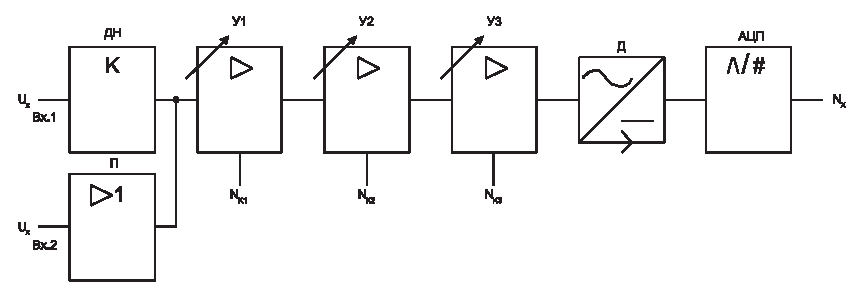
\includegraphics[width=1\linewidth]{./about/func_in}
\caption{}
\label{ris:expe2}
\end{minipage}
\hfill
\begin{minipage}[h]{0.3\linewidth}
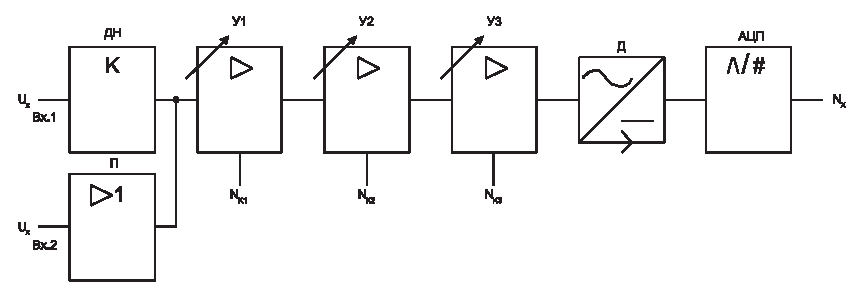
\includegraphics[width=1\linewidth]{./about/func_in}
\caption{}
\label{ris:expe3}
\end{minipage}
\end{center}
\end{figure}






%\subsection{Рисунок, сделанный в LaTeXDraw}

%\begin{pspicture}(0,-1.91)(6.3,1.91)
%\psframe[linewidth=0.04](3.44,0.77)(0.92,-0.77)
%\psframe[linewidth=0.04](4.24,1.07)(2.4,0.09)
%\psline[linewidth=0.04cm](2.76,1.53)(4.06,-0.09)
%\psline[linewidth=0.04cm](6.28,1.19)(0.02,-1.89)
%\psline[linewidth=0.04cm](5.42,1.89)(5.28,-0.07)
%\end{pspicture}


\subsection{Рисунок, сделанный в TikZiT}

Родными файлами этого редактора являются *.tex - файлы, причём компактные и доступные для
понимания/редактирования вручную.

\begin{figure}[H] \centering
\small
% -- Это выхлоп TikZiT, который втягивается обратно при необходимости внести правки >>>>>>>
\begin{tikzpicture}
	\begin{pgfonlayer}{nodelayer}
		\node [style=none] (0) at (-5.25, 13.25) {};
		\node [style=none] (1) at (-2.25, 13.25) {};
		\node [style=none] (2) at (-5.25, 11.75) {};
		\node [style=none] (3) at (-2.25, 11.75) {};
		\node [style=none] (4) at (-3.75, 12.75) {Делитель};
		\node [style=none] (5) at (-3.75, 12.25) {на 3;4;5};
		\node [style=none] (6) at (-7, 12.5) {};
		\node [style=none] (7) at (-5.25, 12.5) {};
		\node [style=none] (9) at (-6.5, 13) {CLK\_I};
		\node [style=none] (10) at (-4.5, 10.25) {};
		\node [style=none] (11) at (-4.5, 11.75) {};
		\node [style=none] (12) at (-3, 10.25) {};
		\node [style=none] (13) at (-3, 11.75) {};
		\node [style=none] (14) at (-5.25, 10.25) {};
		\node [style=none] (15) at (-2.25, 10.25) {};
		\node [style=none] (16) at (-5.25, 6.25) {};
		\node [style=none] (17) at (-2.25, 6.25) {};
		\node [style=none] (18) at (-3.75, 8.75) {Частотно -};
		\node [style=none] (19) at (-3.75, 7.75) {дискриминатор};
		\node [style=none] (23) at (-3.75, 8.25) {фазовый};
		\node [style=none] (24) at (0.75, 12.5) {};
		\node [style=none] (25) at (-2.25, 12.5) {};
		\node [style=none] (27) at (2.25, 13.25) {};
		\node [style=none] (28) at (0.75, 13.25) {};
		\node [style=none] (29) at (3.75, 13.25) {};
		\node [style=none] (30) at (0.75, 11.75) {};
		\node [style=none] (31) at (3.75, 11.75) {};
		\node [style=none] (32) at (2.25, 12.75) {Делитель c};
		\node [style=none] (33) at (2.25, 12.25) {перезагрузкой};
		\node [style=none] (35) at (1.5, 11.75) {};
		\node [style=none] (36) at (3, 11.75) {};
		\node [style=none] (38) at (4.5, 12.5) {};
		\node [style=none] (39) at (4.5, 9.5) {};
		\node [style=none] (40) at (3.75, 9.5) {};
		\node [style=none] (41) at (3.75, 12.5) {};
		\node [style=none] (42) at (-2.25, 9.5) {};
		\node [style=none] (44) at (7, 12.5) {};
		\node [style=none] (47) at (0.75, 10.25) {};
		\node [style=none] (48) at (3.75, 10.25) {};
		\node [style=none] (49) at (0.75, 8.75) {};
		\node [style=none] (50) at (3.75, 8.75) {};
		\node [style=none] (52) at (2.25, 9.25) {на 2};
		\node [style=none] (53) at (0.75, 9.5) {};
		\node [style=none] (54) at (2.25, 9.75) {Делитель};
		\node [style=none] (56) at (6.25, 13) {Частота х2 сфазированная};
		\node [style=none] (59) at (-4, 11) {Inc};
		\node [style=none] (60) at (-2.5, 11) {Dec};
		\node [style=none] (69) at (-2.25, 7) {};
		\node [style=none] (76) at (7, 7) {};
		\node [style=none] (77) at (5.25, 7.5) {Фронты от импульсов};
	\end{pgfonlayer}
	\begin{pgfonlayer}{edgelayer}
		\draw (1.center) to (3.center);
		\draw (0.center) to (1.center);
		\draw (0.center) to (2.center);
		\draw (2.center) to (3.center);
		\draw [style=pointer] (6.center) to (7.center);
		\draw (15.center) to (17.center);
		\draw (14.center) to (15.center);
		\draw (14.center) to (16.center);
		\draw (16.center) to (17.center);
		\draw [style=pointer] (10.center) to (11.center);
		\draw [style=pointer] (12.center) to (13.center);
		\draw [style=pointer] (25.center) to (24.center);
		\draw (29.center) to (31.center);
		\draw (28.center) to (29.center);
		\draw (28.center) to (30.center);
		\draw (30.center) to (31.center);
		\draw (41.center) to (38.center);
		\draw (38.center) to (39.center);
		\draw [style=pointer] (39.center) to (40.center);
		\draw [style=pointer] (38.center) to (44.center);
		\draw (48.center) to (50.center);
		\draw (47.center) to (48.center);
		\draw (47.center) to (49.center);
		\draw (49.center) to (50.center);
		\draw [style=pointer] (53.center) to (42.center);
		\draw [style=pointer] (76.center) to (69.center);
	\end{pgfonlayer}
\end{tikzpicture} 
% <<<<<<<<
\normalsize
\caption{Рисунок, сделанный в TikZiT (какая-то ФАПЧ с непонятным фазовым портретом). Включен в документ как *.tex-код (очень компактный, редактируемый вручную, обратно открываемый TikZiT). Пока авторы делают локализацию, русифицированный TikZiT можно скачать  по ссылке https://github.com/yrasik/tikzit}
\label{ris:image1_TikZiT}
\end{figure}



\subsection{Рисунок, сделанный в Inkscape}

\begin{figure}[H] \centering
\input ./about/inkscape/drawing1.tex
\caption{Рисунок, сделанный в Inkscape. Включен в документ как файл с *.tex-кодом (довольно громоздким), правильно отрисовываются русские буквы, даже растянутые}
\label{ris:image1_ink}
\end{figure}


\subsection{Рисунок, сделанный в Dia}

\begin{figure}[H] \centering
\input ./about/dia/drawing1.tex
\caption{Рисунок, сделанный в Dia. Включен в документ как файл с *.tex-кодом (по сравнению с Inkscape довольно компактный), русские буквы отрисовываются основным шрифтом документа, стрелки на концах линий не так масштабируются}
\label{ris:image1_dia}
\end{figure}



\begin{figure}[H] \centering \fontspec[Scale=2.0]{Times New Roman}
\input ./about/dia/drawing1.tex
\caption{Рисунок, сделанный в Dia. Увеличили шрифт текста прямо в LaTeX}
\label{ris:image1_dia}
\end{figure}








